%%%%%%%%%%%%%%%%%%%%%%%%%%%%%%%%%%%%%%%%%
% Large Colored Title Article
% LaTeX Template
% Version 1.1 (25/11/12)
%
% This template has been downloaded from:
% http://www.LaTeXTemplates.com
%
% Original author:
% Frits Wenneker (http://www.howtotex.com)
%
% License:
% CC BY-NC-SA 3.0 (http://creativecommons.org/licenses/by-nc-sa/3.0/)
%
%%%%%%%%%%%%%%%%%%%%%%%%%%%%%%%%%%%%%%%%%

%----------------------------------------------------------------------------------------
%	PACKAGES AND OTHER DOCUMENT CONFIGURATIONS
%----------------------------------------------------------------------------------------

\documentclass[DIV=calc, paper=a4, fontsize=11pt, twocolumn]{scrartcl}	 % A4 paper and 11pt font size

\usepackage[english]{babel} % English language/hyphenation
\usepackage[protrusion=true,expansion=true]{microtype} % Better typography
\usepackage{amsmath,amsfonts,amsthm} % Math packages
\usepackage[svgnames]{xcolor} % Enabling colors by their 'svgnames'
\usepackage[hang, small,labelfont=bf,up,textfont=it,up]{caption} % Custom captions under/above floats in tables or figures
\usepackage{booktabs} % Horizontal rules in tables
\usepackage{fix-cm}	  % Custom font sizes - used for the initial letter in the document

\usepackage{sectsty}  % Enables custom section titles
\allsectionsfont{\usefont{OT1}{phv}{b}{n}} % Change the font of all section commands

\usepackage{fancyhdr} % Needed to define custom headers/footers
\pagestyle{fancy}     % Enables the custom headers/footers
\usepackage{lastpage} % Used to determine the number of pages in the document (for "Page X of Total")

% Headers - all currently empty
\lhead{}
\chead{}
\rhead{}

% Footers
\lfoot{}
\cfoot{}
\rfoot{\footnotesize Page \thepage\ of \pageref{LastPage}} % "Page 1 of 2"

\renewcommand{\headrulewidth}{0.0pt} % No header rule
\renewcommand{\footrulewidth}{0.4pt} % Thin footer rule

\usepackage{lettrine} % Package to accentuate the first letter of the text
\newcommand{\initial}[1]{ % Defines the command and style for the first letter
\lettrine[lines=3,lhang=0.3,nindent=0em]{
\color{DarkGoldenrod}
{\textsf{#1}}}{}}

%----------------------------------------------------------------------------------------
%	TITLE SECTION
%----------------------------------------------------------------------------------------

\usepackage{titling} % Allows custom title configuration
\newcommand{\HorRule}{\color{DarkGoldenrod} \rule{\linewidth}{1pt}} % Defines the gold horizontal rule around the title
\pretitle{\vspace{-30pt} \begin{flushleft} \HorRule \fontsize{50}{50} \usefont{OT1}{phv}{b}{n} \color{DarkRed} \selectfont} % Horizontal rule before the title
\title{Detection of Coffee Seeds in Images by the Color} % Your article title
\posttitle{\par\end{flushleft}\vskip 0.5em} % Whitespace under the title
\preauthor{\begin{flushleft}\large \lineskip 0.5em \usefont{OT1}{phv}{b}{sl} \color{DarkRed}} % Author font configuration
\author{Fernando Pujaico Rivera, } % Your name
\postauthor{\footnotesize \usefont{OT1}{phv}{m}{sl} \color{Black} % Configuration for the institution name
University of Lavras% Your institution
\par\end{flushleft}\HorRule} % Horizontal rule after the title
\date{} % Add a date here if you would like one to appear underneath the title block


%----------------------------------------------------------------------------------------
%----------------------------------------------------------------------------------------
%----------------------------------------------------------------------------------------
%----------------------------------------------------------------------------------------
%----------------------------------------------------------------------------------------
%----------------------------------------------------------------------------------------

\usepackage{comment}

\usepackage{biblatex}
\addbibresource{section1.bib}

\usepackage{hyperref}
\hypersetup{
    colorlinks=true,
    linkcolor=DarkRed,
    filecolor=magenta,      
    urlcolor=green,
    pdftitle={Fernando Pujaico Rivera},
    bookmarks=true,
}

\usepackage{graphicx}

%----------------------------------------------------------------------------------------
%----------------------------------------------------------------------------------------

\newcommand{\showfont}{codifica\c{c}\~ao: \f@encoding{},
  familia: \f@family{},
  serie: \f@series{},
  %shape: \f@shape{},
  e tamanho: \f@size{} pt
}

%%%%%%%%%%%%%%%%%%%%%%%%%%%%%%%%%%%%%%%%%%%%%%%%%%%%%%%%%%%%%%%%%%%%%%%%%%%%%%%%
%%%%%%%%%%%%%%%%%%%%%%%%%%%%%%%%%%%%%%%%%%%%%%%%%%%%%%%%%%%%%%%%%%%%%%%%%%%%%%%%
%%%% Macros para equaçoes
%%%%%%%%%%%%%%%%%%%%%%%%%%%%%%%%%%%%%%%%%%%%%%%%%%%%%%%%%%%%%%%%%%%%%%%%%%%%%%%%
\newcommand{\Wellposed}{Bem-posto}
\newcommand{\wellposed}{bem-posto}
\newcommand{\Illposed}{Mal-posto}
\newcommand{\illposed}{mal-posto}


%% ARCMIN
%%\newcommand{\argmin}[1]{{\operatorname{arg}_{#1}\operatorname{min}}\;}

%% morepenrose function
\newcommand{\getminparam}{\operatorname{get}\_\operatorname{poly2}\_\operatorname{coefs}}

%% diagonal function
\newcommand{\funcnumel}{numel}

%% diagonal function
\newcommand{\funcdiag}{diag}


%% vectorization function
\newcommand{\funcvec}{vec}

%% transpose function
\newcommand{\funcinv}{inv}

%% transpose function
\newcommand{\functrans}{trans}
%% transpose operator
\newcommand{\transpose}{\mathrm{T}}

%% Time of sampling
\newcommand{\ToS}{\tau}

%% block matrix
%\newcommand{\funcblockdiag}{blkdiag}
%\newcommand{\funcblockhor }{blkhorz}
%\newcommand{\funcblockver }{blkvert}


%% definiçao de tipos de arrays
\newcommand{\TRIX}[1]{\mathbf{\overline{\uppercase{#1}}}}
\newcommand{\MATRIX}[1]{\mathbf{\uppercase{#1}}}
\newcommand{\VECTOR}[1]{\mathbf{\lowercase{#1}}}
\newcommand{\DTVECTOR}[1]{\mathbf{\dot{\lowercase{#1}}}}
\newcommand{\DDTVECTOR}[1]{\mathbf{\ddot{\lowercase{#1}}}}
\newcommand{\DDDTVECTOR}[1]{\mathbf{\dddot{\lowercase{#1}}}}
\newcommand{\DDDDTVECTOR}[1]{\mathbf{\ddddot{\lowercase{#1}}}}
%%%%%%%%%%%%%%%%%%%%%%%%%%%%%%%%%%%%%%%%%%%%%%%%%%%%%%%%%%%%%%%%%%%%%%%%%%%%%%%%
%%%%%%%%%%%%%%%%%%%%%%%%%%%%%%%%%%%%%%%%%%%%%%%%%%%%%%%%%%%%%%%%%%%%%%%%%%%%%%%%
%%%% Macros para texto
%%%%%%%%%%%%%%%%%%%%%%%%%%%%%%%%%%%%%%%%%%%%%%%%%%%%%%%%%%%%%%%%%%%%%%%%%%%%%%%%

\newcommand{\FALTAPROVA}{\textcolor{red}{[FALTA PROVA!!!]}}
\newcommand{\FALTAREFERENCIA}{\textcolor{red}{[FALTA REFERENCIA!!!]}}

\usepackage[]{algorithm2e}

\begin{document}

\maketitle % Print the title

\thispagestyle{fancy} % Enabling the custom headers/footers for the first page 

%----------------------------------------------------------------------------------------
%	ABSTRACT
%----------------------------------------------------------------------------------------

% The first character should be within \initial{}
\initial{H}\textbf{ere is presented a 
techniques to the detection of coffee seeds by the use of $RGB$ pixel color.}

%----------------------------------------------------------------------------------------
%	ARTICLE CONTENTS
%----------------------------------------------------------------------------------------
\section{Data set and model}
The main problem, in this work, consist into 
detect the coffee seeds  in a picture like the showed in Fig. \ref{fig:data-color}.
\begin{figure}[h!]
\centering
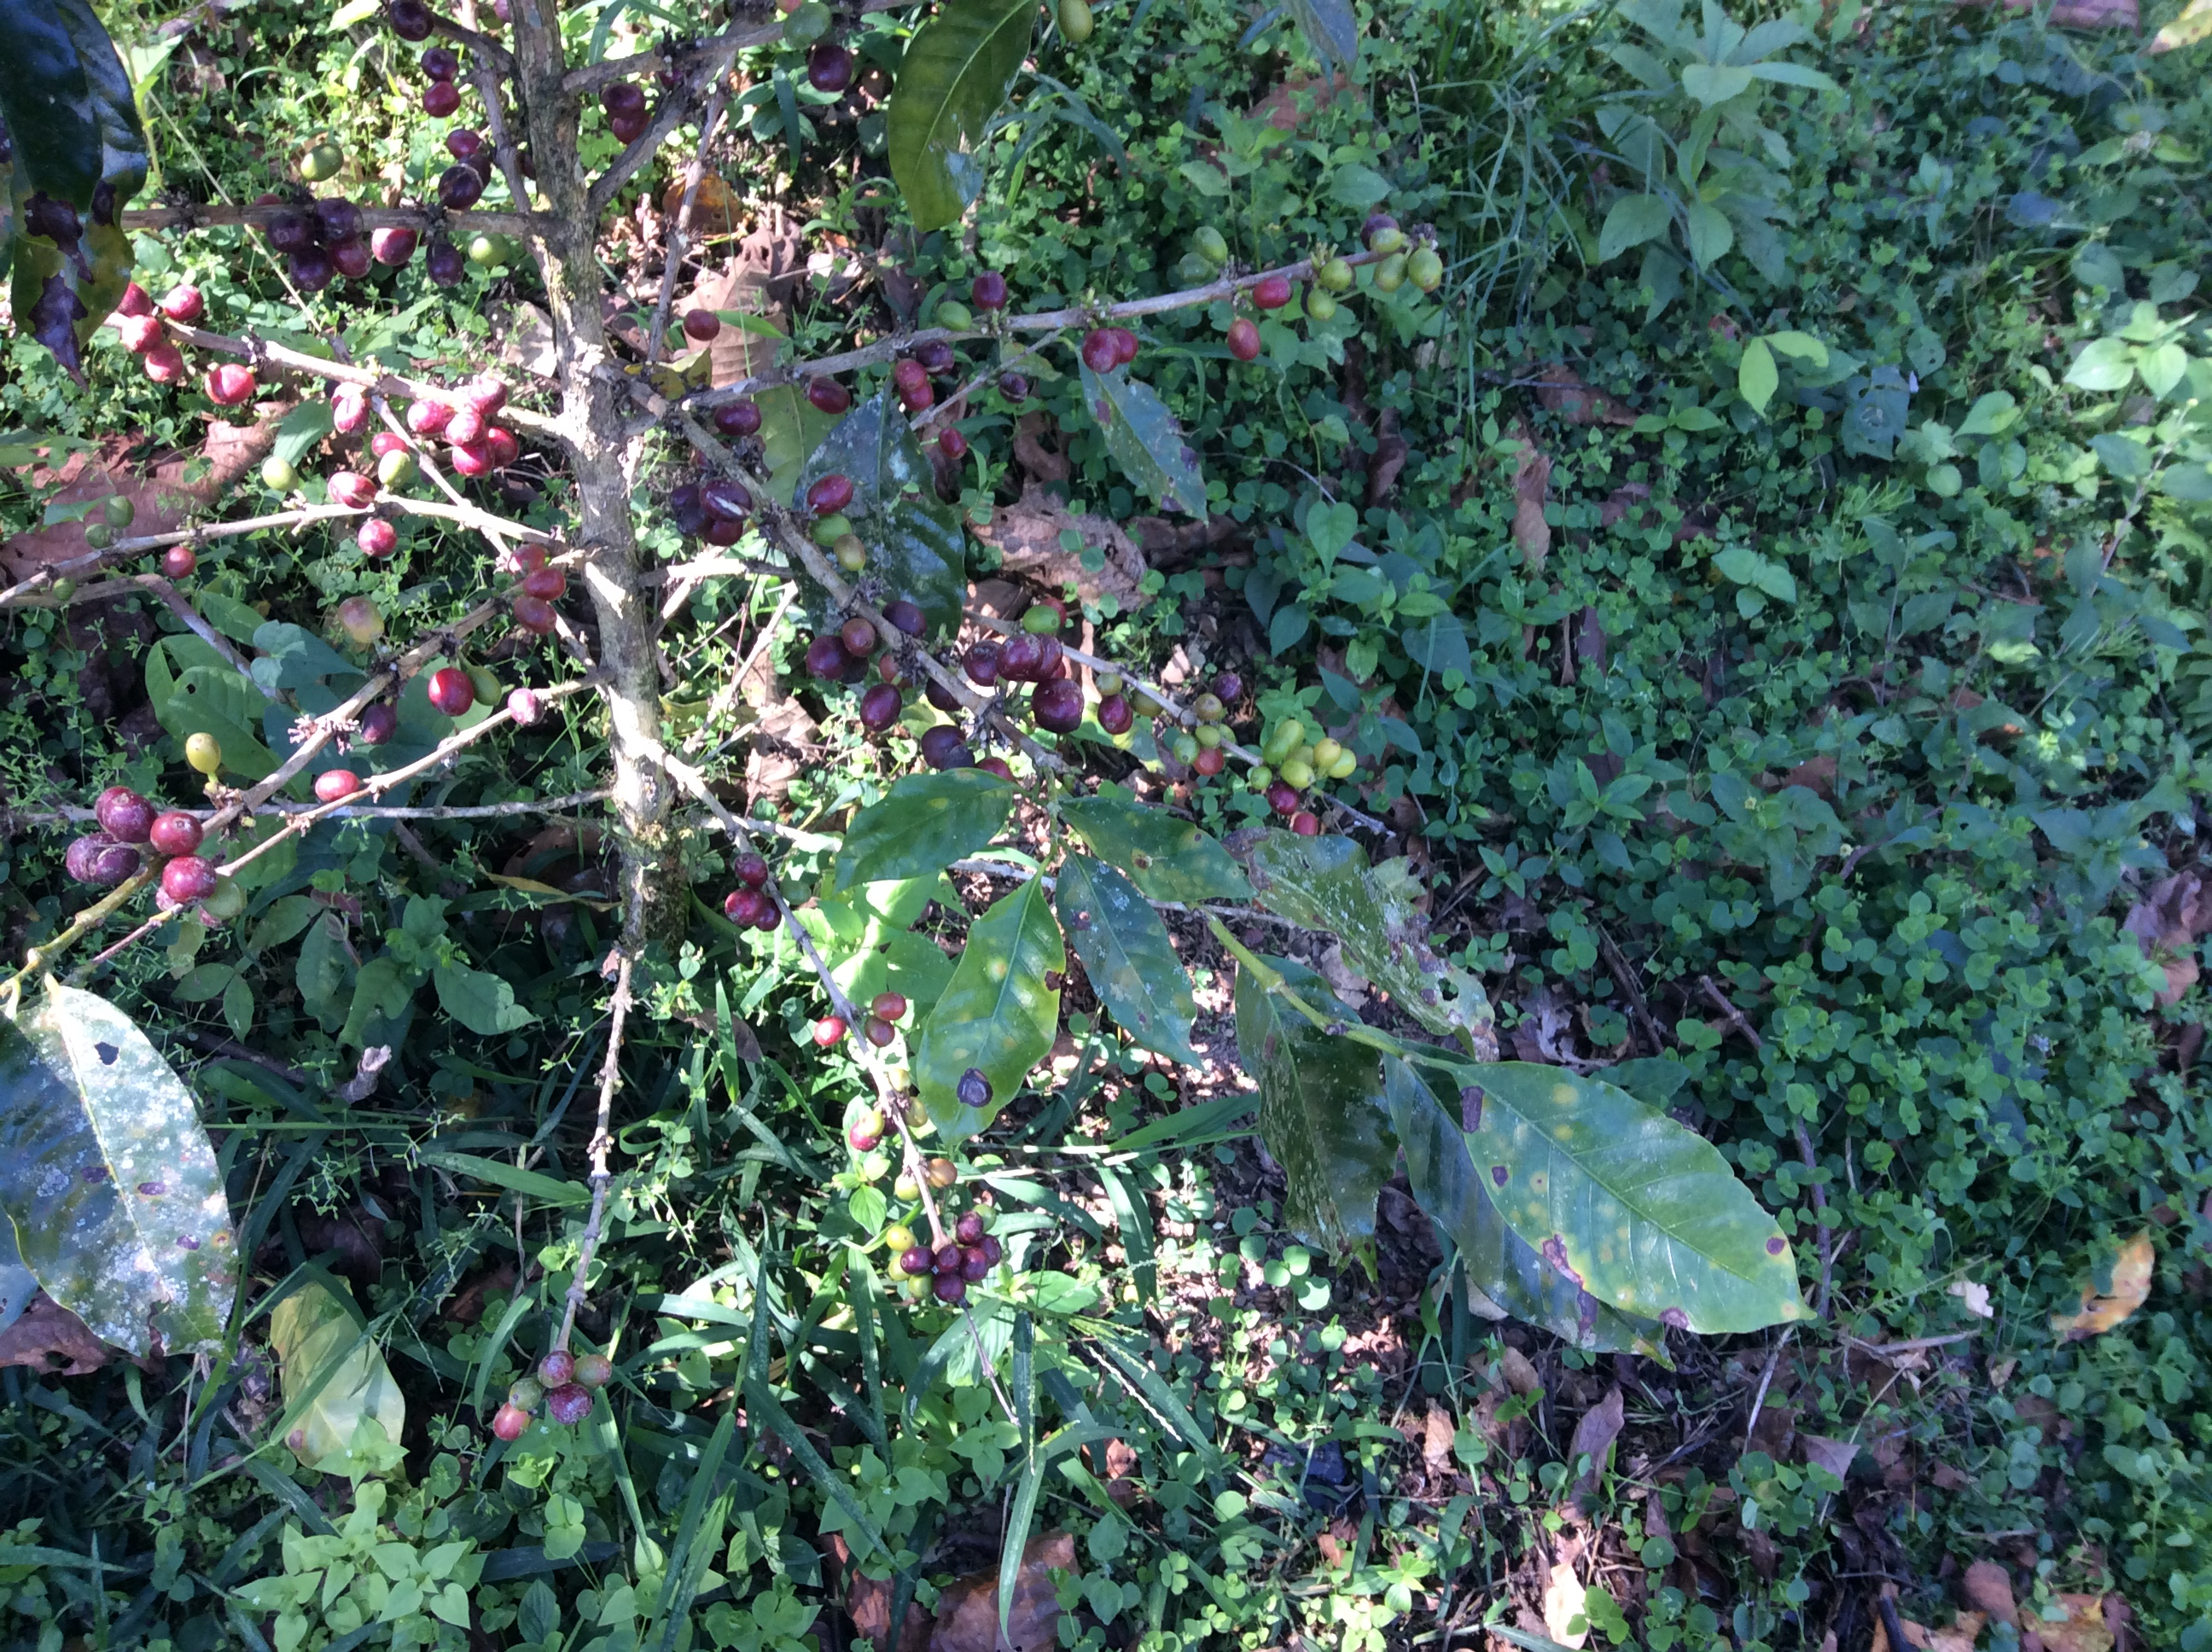
\includegraphics[width=0.99\linewidth]{IMG_0225.JPG}
\caption{Source image.}
\label{fig:data-color}
\end{figure} 

\subsection{Model}
Here a classification model is proposed through the function
$f_{\VECTOR{c}}:~\mathbb{R}^{3} \rightarrow \mathbb{R}$,
\begin{equation}
f_{\VECTOR{c}}(\VECTOR{x})=\frac{1}{1+e^{-h_{\VECTOR{c}}(\VECTOR{x})}},
\end{equation}
\begin{equation}
h_{\VECTOR{c}}(\VECTOR{x}) = c_1+c_2 x_1+c_3 x_2+c_4 x_3,
\end{equation}
where the column vector $\VECTOR{x}\in \mathbb{R}^{3}$ represents a pixel,
 with the $RGB$ additive color model,
 $\VECTOR{x}=[x_1,~ x_2,~ x_3]^{\transpose}\equiv [red,~ green,~ blue]^{\transpose}$
in the Fig. \ref{fig:data-color};
thus, the value $y=f_{\VECTOR{c}}(\VECTOR{x})$ indicates the state or label 
of sample $\VECTOR{x}$.
We consider that all color points  in the Fig. \ref{fig:data-color}
are separated principally in two sets (states); 
one set with color points that belong to a coffee seed,
with $y$ values close to $1$,
and another with everyone who doesn't belong, with $y$ values close to $0$.
The use of kernel function $h_{\VECTOR{c}}(\VECTOR{x})$ 
indicates that we assume that we can separate (approximately) 
these two sets by the hyper-plane $h_{\VECTOR{c}}(\VECTOR{x})=0$.

The function $f_{\VECTOR{c}}(\VECTOR{x})$, that is a modification of a sigmoid function,
has the characteristic that returns values between $0$ and $1$,
being that take a value $0.5$ when $h_{\VECTOR{c}}(\VECTOR{x})=0$;
%We consider that the function $f_{\VECTOR{c}}(\VECTOR{x})$ take values close to $1$
%when the color belong to a coffee seed, and the values close to $0$ when not;
%intermediate values indicates intermediate certainties;
remembering that the function $f_{\VECTOR{c}}(\VECTOR{x})$ only reaches $0$ and $1$ at $-\infty$ and $+\infty$,
respectively;
thus, our objective in the next sections will be found the column vector $\VECTOR{c}\in \mathbb{R}^{4}$,
where $\VECTOR{c}=[c_1,~ c_2,~ c_3,~ c_4]^{\transpose}$, that characterize the function $f_{\VECTOR{c}}(\VECTOR{x})$.

\subsection{Training}

To get the parameter vector $\VECTOR{c}=[c_1,~ c_2,~ c_3,~ c_4]^{\transpose}$
of function $f_{\VECTOR{c}}(\VECTOR{x})$, 
we need a set of training data like shown in the Fig. \ref{fig:data-trainning-bw},
\begin{figure}[h!]
\centering
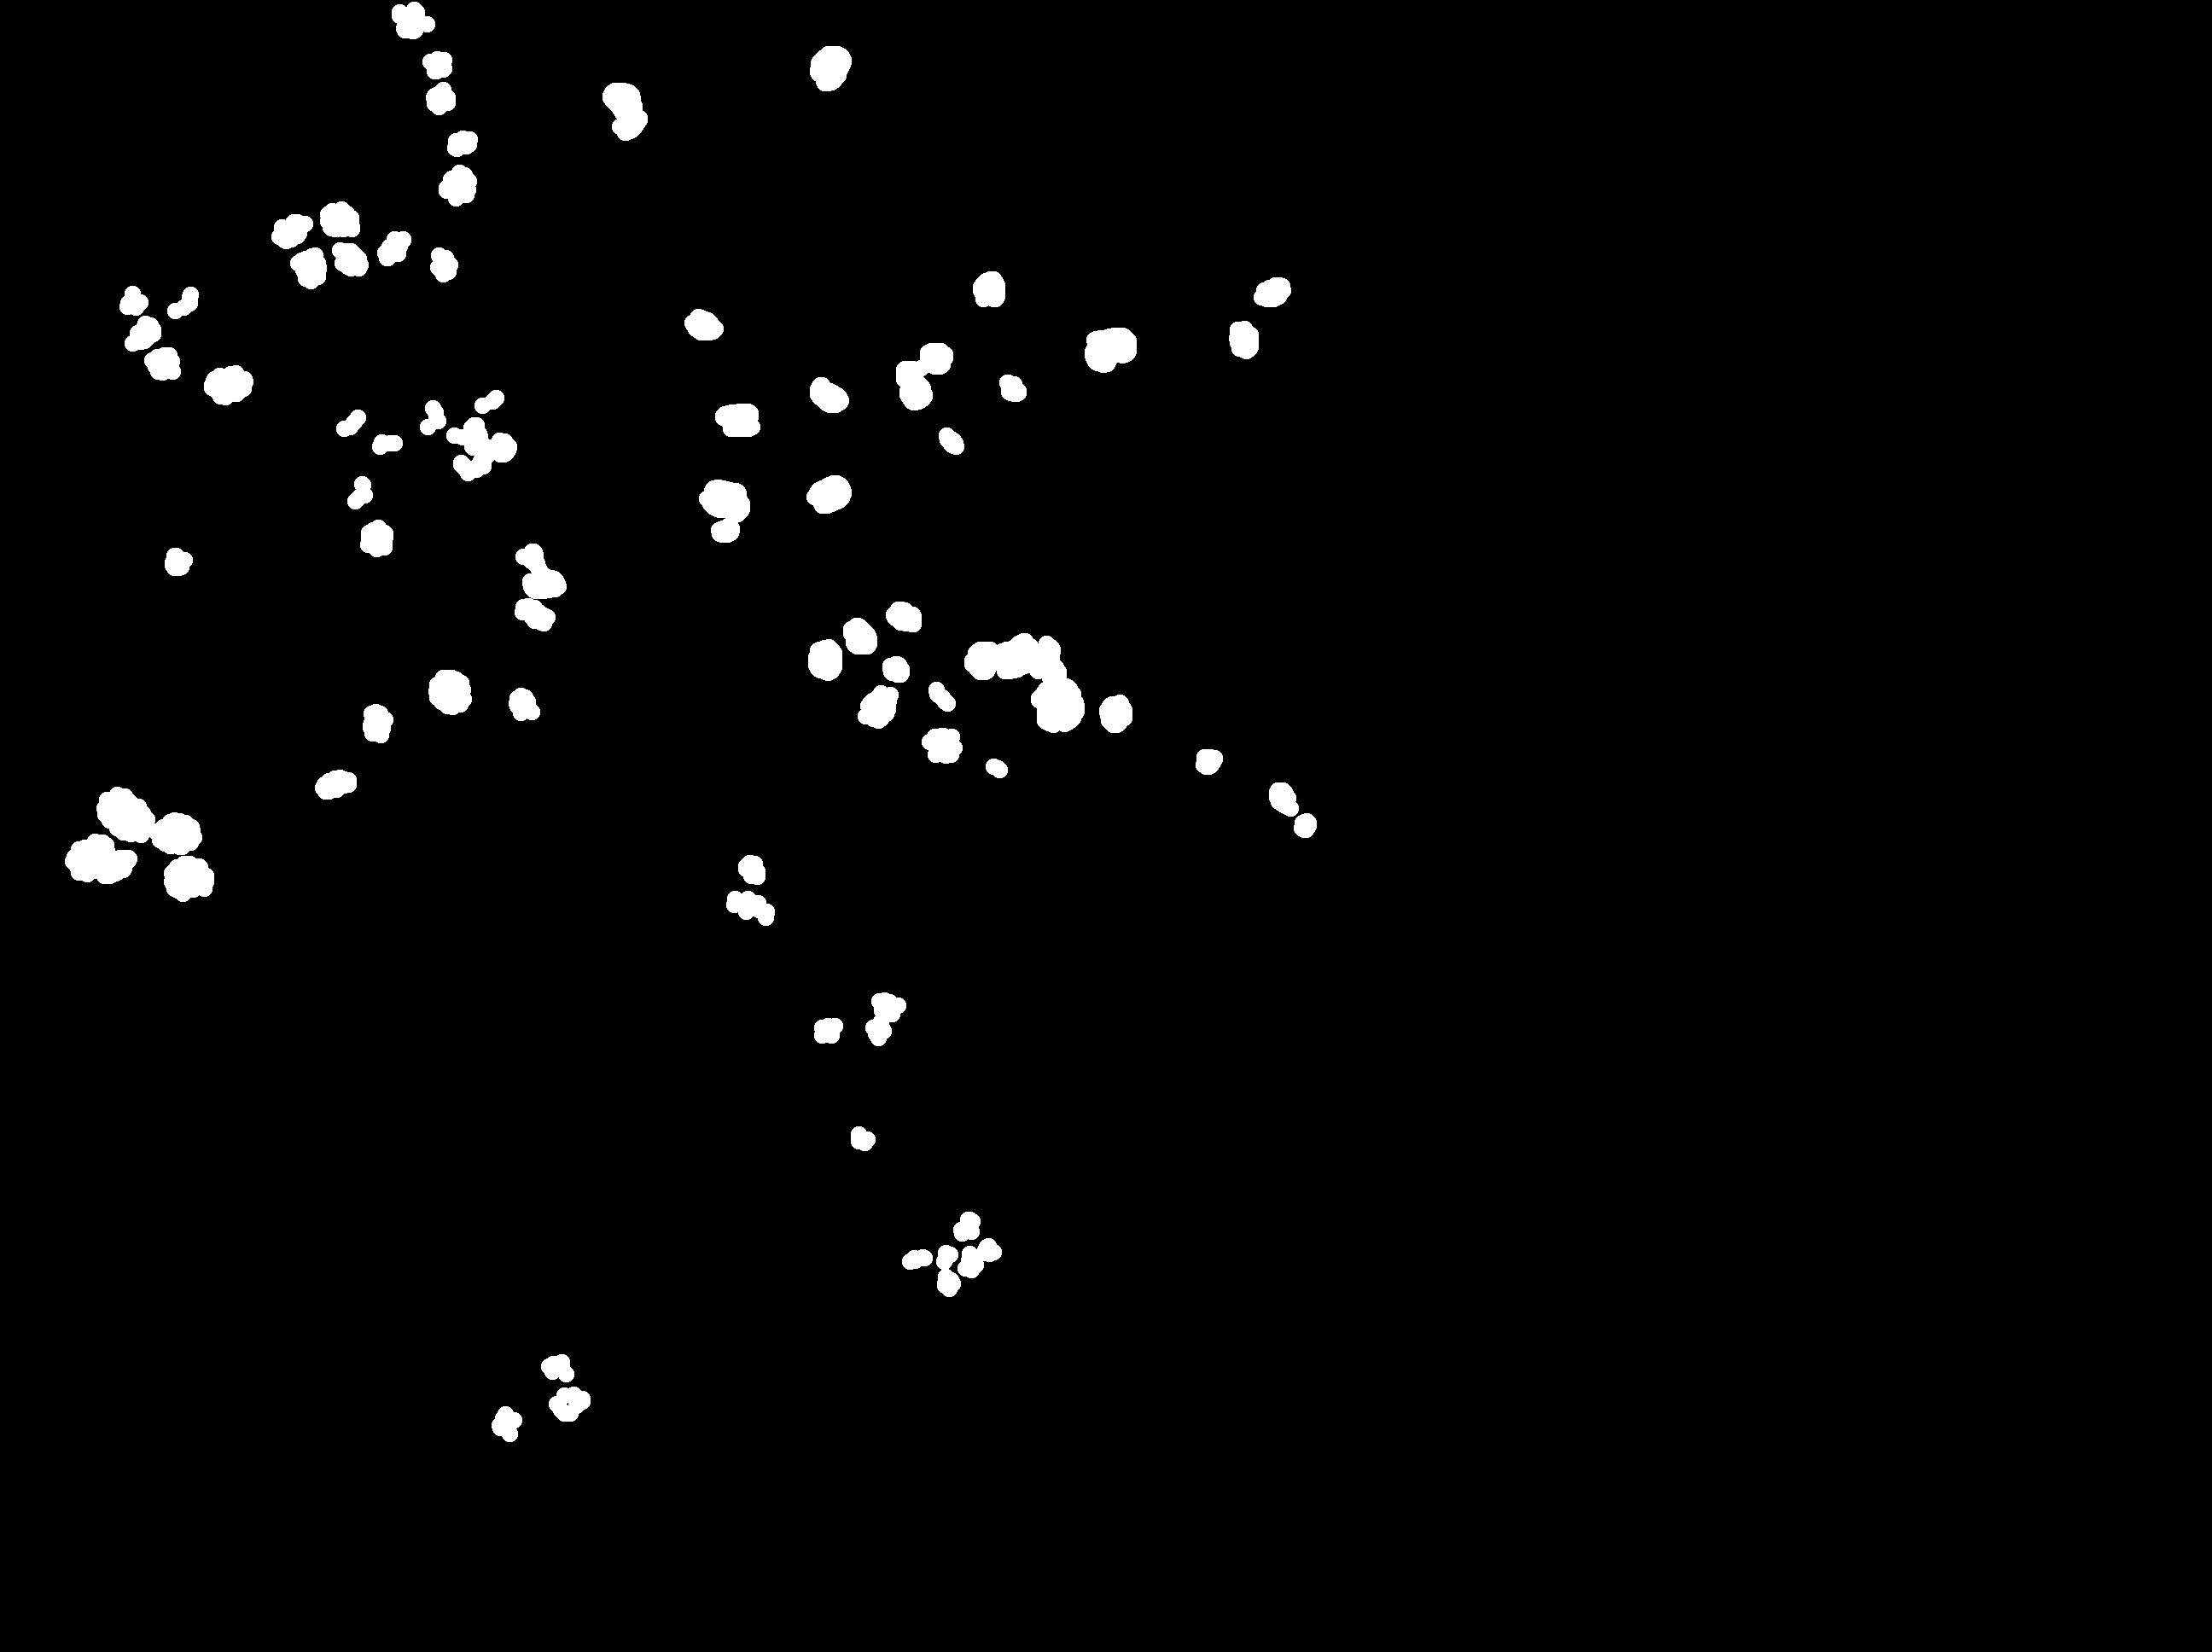
\includegraphics[width=0.99\linewidth]{IMG_0225-BW.png}
\caption{Training data.}
\label{fig:data-trainning-bw}
\end{figure} 
where the picture indicates with the white pixels, the approximate 
location\footnote{Manually painted.} of coffee seeds,
and the black pixels where not. 

Thus, using the pictures of Fig \ref{fig:data-color} and \ref{fig:data-trainning-bw},
we can training the model proposed in the function $f_{\VECTOR{c}}(\VECTOR{x})$
to get the vector $\VECTOR{c}=\VECTOR{\hat{c}}$
that optimizes the fit of training information.



\section{Training the model $f_{\VECTOR{c}}(\VECTOR{x})$}

When we training the model $f_{\VECTOR{c}}(\VECTOR{x})$
our objective is found the vector $\VECTOR{c}=\VECTOR{\hat{c}}$, with the parameters of model, 
that minimise the error when we try fit the model with the training information.
This information is located in 
\begin{itemize}
\item $\MATRIX{I}_c$: The colour image shown in Fig. \ref{fig:data-color}.
\item $\MATRIX{I}_{bw}$: The black and white image shown in Fig. \ref{fig:data-trainning-bw}.
\end{itemize}
The Fig \ref{fig:training} represents this procedure.

\begin{figure}[h!]
\centering
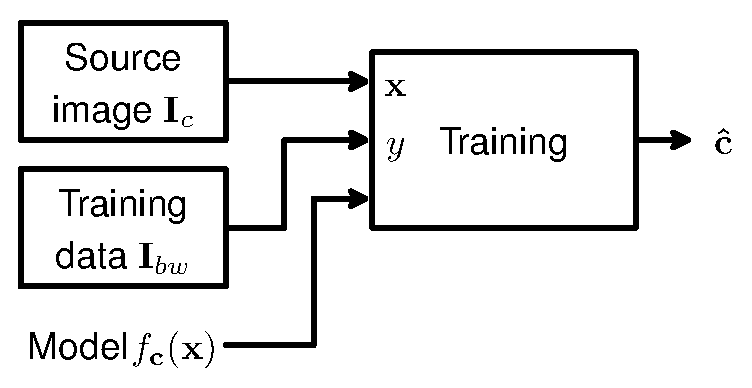
\includegraphics[width=0.99\linewidth]{training.eps}
\caption{Block diagram of model training.}
\label{fig:training}
\end{figure} 

The training block follow the procedure described in the 
Algorithm \ref{alg:alg1}, that additionally need some variables like $\epsilon=0.00005$, $N=11023$ and $K=10$ to work.
\begin{itemize}
\item $\epsilon$: The value $y$ to each pixel $\VECTOR{x}$ chosen in image $\MATRIX{I}_{c}$
with a ``black'' pixel in image $\MATRIX{I}_{bw}$, where $0 < \epsilon \ll 0.5$.
\item $N$: The number of randomly selected points (pixels) 
in each training repetition.
\item $K$: The number of training repetitions.
\end{itemize}

\begin{algorithm}
 \KwData{
$\MATRIX{I}_c$,
$\MATRIX{I}_{bw}$,
$\epsilon$,
$N$,
$K$.
}
 \KwResult{The optimised $\VECTOR{\hat{c}}$ parameter to form the classifier $f_{\VECTOR{\hat{c}}}(\VECTOR{x})$.}~\\
 $\VECTOR{y}=[\underbrace{\epsilon   \quad \hdots \quad \epsilon }_{N~elements} \quad 
\underbrace{ 1-\epsilon \quad \hdots \quad 1-\epsilon }_{N~elements}]^{\transpose}$\;
 \For{$k=1$ \KwTo $K$}{
  $\MATRIX{P}_b=get\_points(\MATRIX{I}_c,\MATRIX{I}_{bw},N,``\mathbf{black}")$\;
  $\MATRIX{P}_w=get\_points(\MATRIX{I}_c,\MATRIX{I}_{bw},N,``\mathbf{white}")$\;
  $\MATRIX{P}=\begin{bmatrix}\MATRIX{P}_b\\ \MATRIX{P}_w \end{bmatrix}$\;
  $\left[\VECTOR{\hat{c}}_k,~e(\VECTOR{\hat{c}}_k)\right]=get\_parameters\left( \MATRIX{P}, \VECTOR{y}\right)$\;
 }
 $\VECTOR{\hat{c}}=\frac{\sum\limits_{k=1}^{K} \frac{\VECTOR{\hat{c}}_k}{e(\VECTOR{\hat{c}}_k)}}{\sum\limits_{k=1}^{K} \frac{1}{e(\VECTOR{\hat{c}}_k)}}$\;
 \caption{Method to get the vector $\VECTOR{\hat{c}}$.}
\label{alg:alg1}
\end{algorithm}

\subsection{Function $get\_points(\MATRIX{I}_c,\MATRIX{I}_{bw},N,TYPE)$}
The function choose randomly\footnote{Follow an uniform distribution.}
$N$ points (pixels) $\VECTOR{x}_n$, $1 \leq n \leq N$,
from the colour image $\MATRIX{I}_c$,
with the condition that each point selected in $\MATRIX{I}_c$ need be of type $TYPE$
in the same position of image $\MATRIX{I}_{bw}$;
where $TYPE \in \{``\mathbf{black}",``\mathbf{white}"\}$. 
Thus, the function return the matrix $\MATRIX{P} \in \mathbb{R}^{N \times 3}$,
\begin{equation}
\MATRIX{P}=
\begin{bmatrix}
\VECTOR{x}_1^{\transpose}  \\
%\VECTOR{x}_2^{\transpose}  \\
\vdots  \\
\VECTOR{x}_n^{\transpose}  \\
\vdots \\
\VECTOR{x}_N^{\transpose} \\
\end{bmatrix},
\end{equation} 
with the information of $N$ randomly selected black or white points.

\subsection{Function $get\_parameters\left( \MATRIX{P}, \VECTOR{y}\right)$}
Given, a group of $L$ points
$\VECTOR{x}_l \in \mathbb{R}^{3}$,
labelled with the values $y_l \in \mathbb{R}$, $1\leq l \leq L$;
ordering in the matrices $\MATRIX{P} \in \mathbb{R}^{L \times 3}$ and 
$\VECTOR{Y} \in \mathbb{R}^{L}$ respectively,
\begin{equation}
\MATRIX{P}=
\begin{bmatrix}
\VECTOR{x}_1^{\transpose}  \\
%\VECTOR{x}_2^{\transpose}  \\
\vdots  \\
\VECTOR{x}_l^{\transpose}  \\
\vdots \\
\VECTOR{x}_L^{\transpose} \\
\end{bmatrix},
\quad 
\VECTOR{y}=
\begin{bmatrix}
y_1  \\
%y_2  \\
\vdots  \\
y_l  \\
\vdots \\
y_L \\
\end{bmatrix};
\end{equation}
if we want to create a classifier using the function $f_{\VECTOR{c}}(\VECTOR{x})$,
with domain $\VECTOR{x} \in \mathbb{R}^{3}$, range $y \in \mathbb{R}$ and
parameters grouped in the vector $\VECTOR{c}\in \mathbb{R}^{4}$,
as defined in Eq. (\ref{eq:reglogrnr1:1}),
\begin{equation}\label{eq:reglogrnr1:1}
y=f_{\VECTOR{c}}(\VECTOR{x}),
\end{equation}
or your equivalent
\begin{equation}\label{eq:logitfunc}
logit(y)=h_{\VECTOR{c}}(\VECTOR{x}),
\end{equation}
where $logit(y) \equiv ln\left( \frac{y}{1-y}\right)$.
We can affirm that 
the vector $\VECTOR{c}= \VECTOR{\hat{c}}$
that fit the model $f_{\VECTOR{c}}$ between the samples $\VECTOR{x}_l$ and the labels $y_l$,
and minimise the square error $e(\VECTOR{c})$,
\begin{equation}\label{eq:reglogrnr1:1e}
\begin{array}{lll}
e(\VECTOR{c}) & = & \frac{1}{L}\sum\limits_{l=1}^{L} ||h_{\VECTOR{c}}(\VECTOR{x}_l)-logit(y_l)||^2,\\
            ~ & = & \frac{1}{L}\sum\limits_{l=1}^{L} ||\left[1\quad \VECTOR{x}_l^{\transpose}\right]\VECTOR{c}-logit(y_l)||^2,\\
            ~ & = & \frac{1}{L}||\MATRIX{A}\VECTOR{c}-\VECTOR{z}||^2,
\end{array}
\end{equation}
\begin{equation}
\MATRIX{A}=
\begin{bmatrix}
1 & \VECTOR{x}_1^{\transpose}\\
%1 & \VECTOR{x}_2^{\transpose}\\
\vdots & \vdots\\
1 & \VECTOR{x}_l^{\transpose}\\
\vdots & \vdots\\
1 & \VECTOR{x}_L^{\transpose}\\ 
\end{bmatrix},
\quad
\VECTOR{z}=
\begin{bmatrix}
logit(y_1)  \\
%logit(y_2)  \\
\vdots  \\
logit(y_l)  \\
\vdots \\
logit(y_L) \\
\end{bmatrix},
\end{equation}
can be found by the Eq. (\ref{eq:reglogrnr1:2}), 
\begin{equation}\label{eq:reglogrnr1:2}
\VECTOR{\hat{c}} = \left[ \MATRIX{A}^{\transpose} \MATRIX{A}\right]^{-1} \MATRIX{A}^{\transpose} \VECTOR{z},\\
\end{equation}
and affirm that $[\VECTOR{\hat{c}},~e(\VECTOR{\hat{c}})]=get\_parameters\left( \MATRIX{P}, \VECTOR{y}\right)$.


\section{Results}
Following the procedure described in the Algorithm \ref{alg:alg1},
we can obtain the vector $\VECTOR{\hat{c}}$ that optimize the model fitting of 
$f_{\VECTOR{\hat{c}}}(\VECTOR{x})$ between the training information;
so that
\begin{equation}
\VECTOR{\hat{c}}=
\begin{bmatrix}
0.13510 & -0.24261 &  0.10244 & -1.95836
\end{bmatrix},
\end{equation}
and consequently
\begin{equation}
f_{\VECTOR{\hat{c}}}(\VECTOR{x})=\frac{1}{1+e^{-0.13510 + 0.24261 x_1 -0.10244 x_2 + 1.95836 x_3}}.
\end{equation}

A Fig. \ref{fig:planecoef} shows two sets, of $N$ points each one, 
selected randomly in the Fig. \ref{fig:data-trainning-bw},
the points $\VECTOR{x}$ drawn with the color red represent pixels in a coffee seeds, and
the points $\VECTOR{x}$ drawn with the color blue represent pixels that don't belong to a coffee seed.

\begin{figure}[h!]
\centering
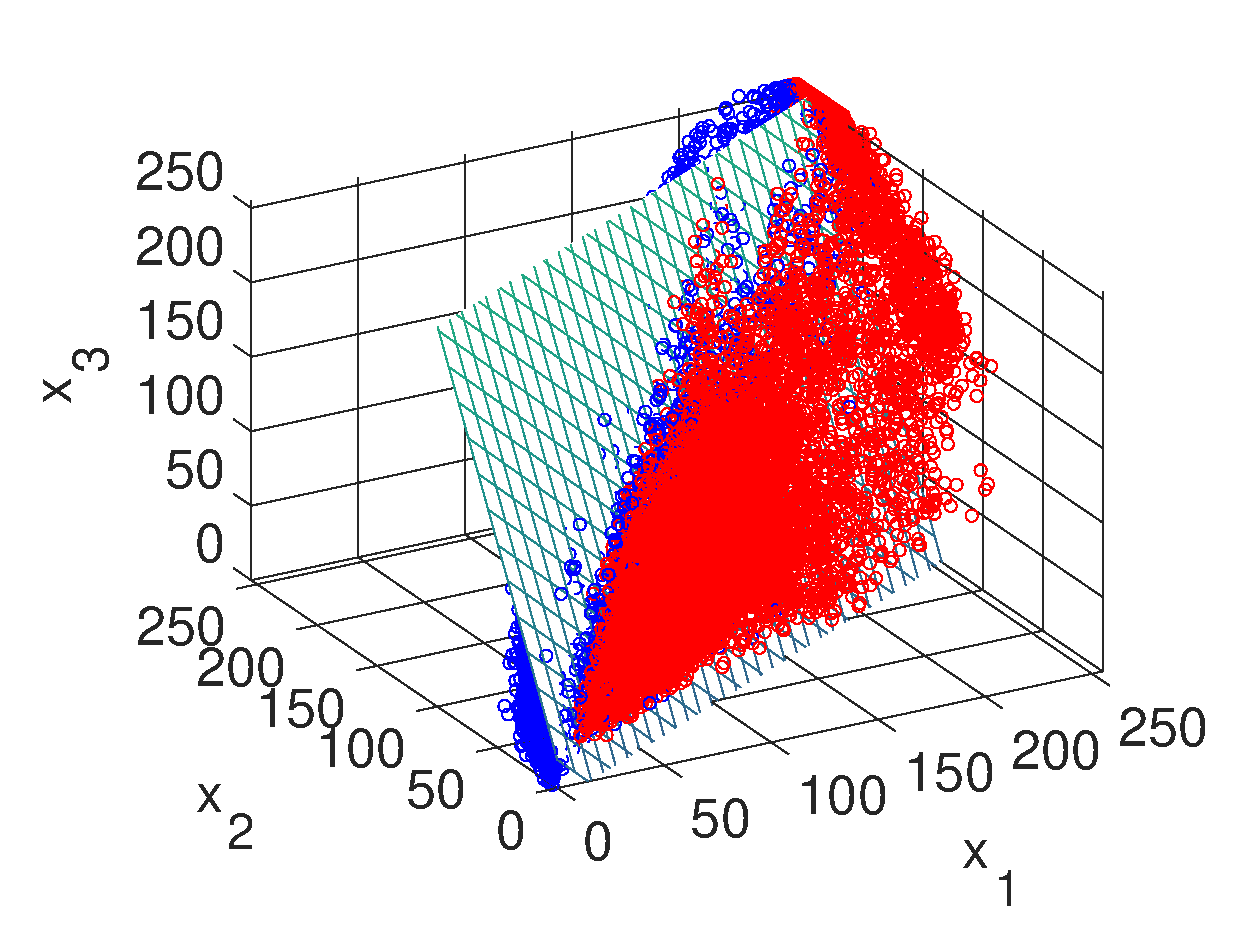
\includegraphics[width=0.99\linewidth]{plane_coef.eps}
\caption{Points $\VECTOR{x} \in \mathbb{R}^{3}$ and the hyperplane $h_{\VECTOR{\hat{c}}}(\VECTOR{x})=0$.}
\label{fig:planecoef}
\end{figure} 

The Fig. \ref{fig:sigmoid_result} shows the result of evaluate each pixel $\VECTOR{x}$ of Fig. \ref{fig:data-color}
with the function $f_{\VECTOR{\hat{c}}}(\VECTOR{x})$.
Thus, the resulting image have values between $0$ and $1$,
and was colorized with a color map with colors between blue and red 
to show results $0<y<1$.
\begin{figure}[h!]
\centering
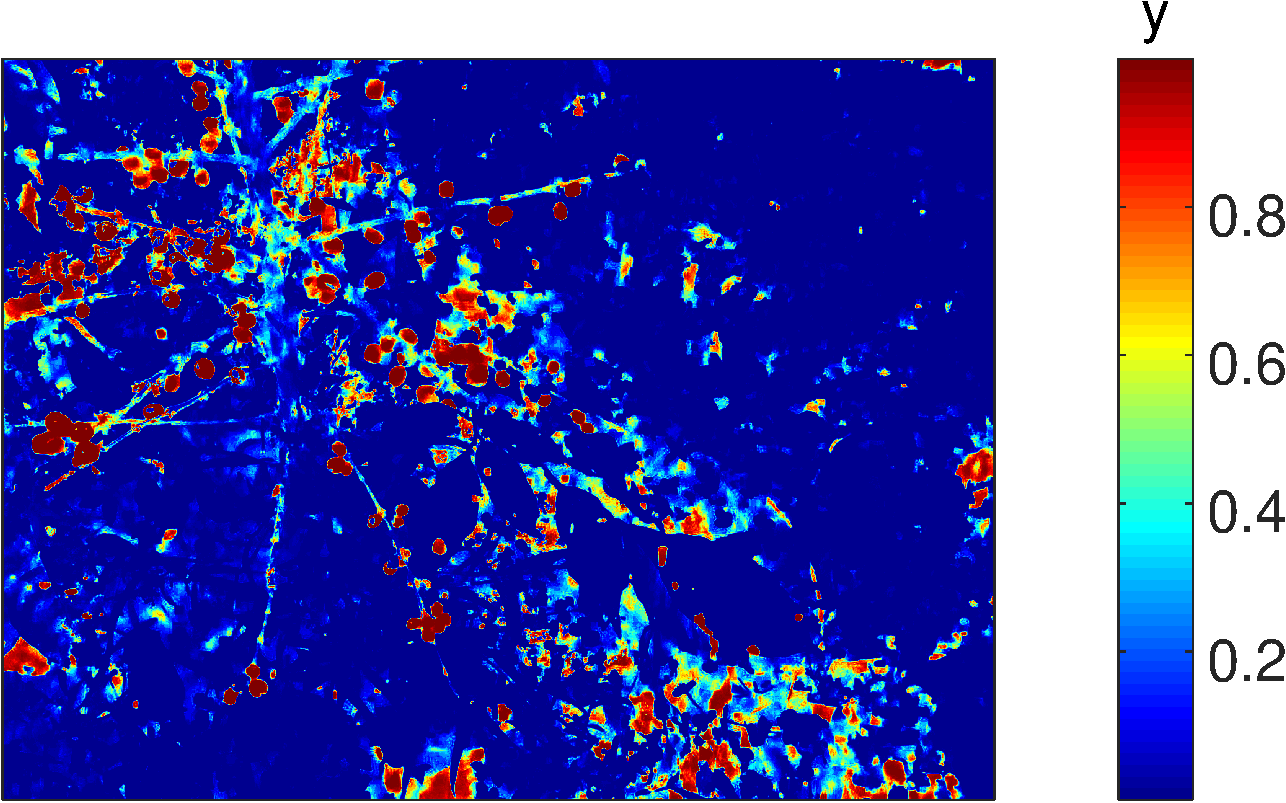
\includegraphics[width=0.99\linewidth]{sigmoid_result.png}
\caption{Result of function $f_{\VECTOR{\hat{c}}}(\VECTOR{x})$.}
\label{fig:sigmoid_result}
\end{figure} 

%----------------------------------------------------------------------------------------
%	REFERENCE LIST
%----------------------------------------------------------------------------------------

\printbibliography

%----------------------------------------------------------------------------------------

\end{document}
